\documentclass[border=12pt]{standalone}

\usepackage[T1]{fontenc}
\usepackage{amsmath}
\usepackage{amssymb}
\usepackage{xcolor}
\usepackage{tikz}
\usetikzlibrary{arrows.meta,positioning,shapes.geometric,fit,backgrounds,calc}

% ---------- shorthand ----------
\newcommand{\Etot}{E_{\mathrm{tot}}}
\newcommand{\Etr}{E_{\mathrm{tr}}}
\newcommand{\Erot}{E_{\mathrm{rot}}}
\newcommand{\etatr}{\eta_{\mathrm{tr}}}
\newcommand{\etarot}{\eta_{\mathrm{rot},A}}
\newcommand{\xv}{\mathbf{x}}
\newcommand{\yv}{\mathbf{y}}

% ---------- colours ----------
\definecolor{trainbg}{HTML}{EEF3FA}
\definecolor{trainln}{HTML}{6E86A8}
\definecolor{dsmcbg}{HTML}{F6F2EA}
\definecolor{dsmcln}{HTML}{A88E63}
\definecolor{mdnfill}{HTML}{D6EBE8}
\definecolor{mdnline}{HTML}{2E7D74}
\definecolor{nodeln}{HTML}{3A3A3A}
\definecolor{accent}{HTML}{B23A48}

\begin{document}
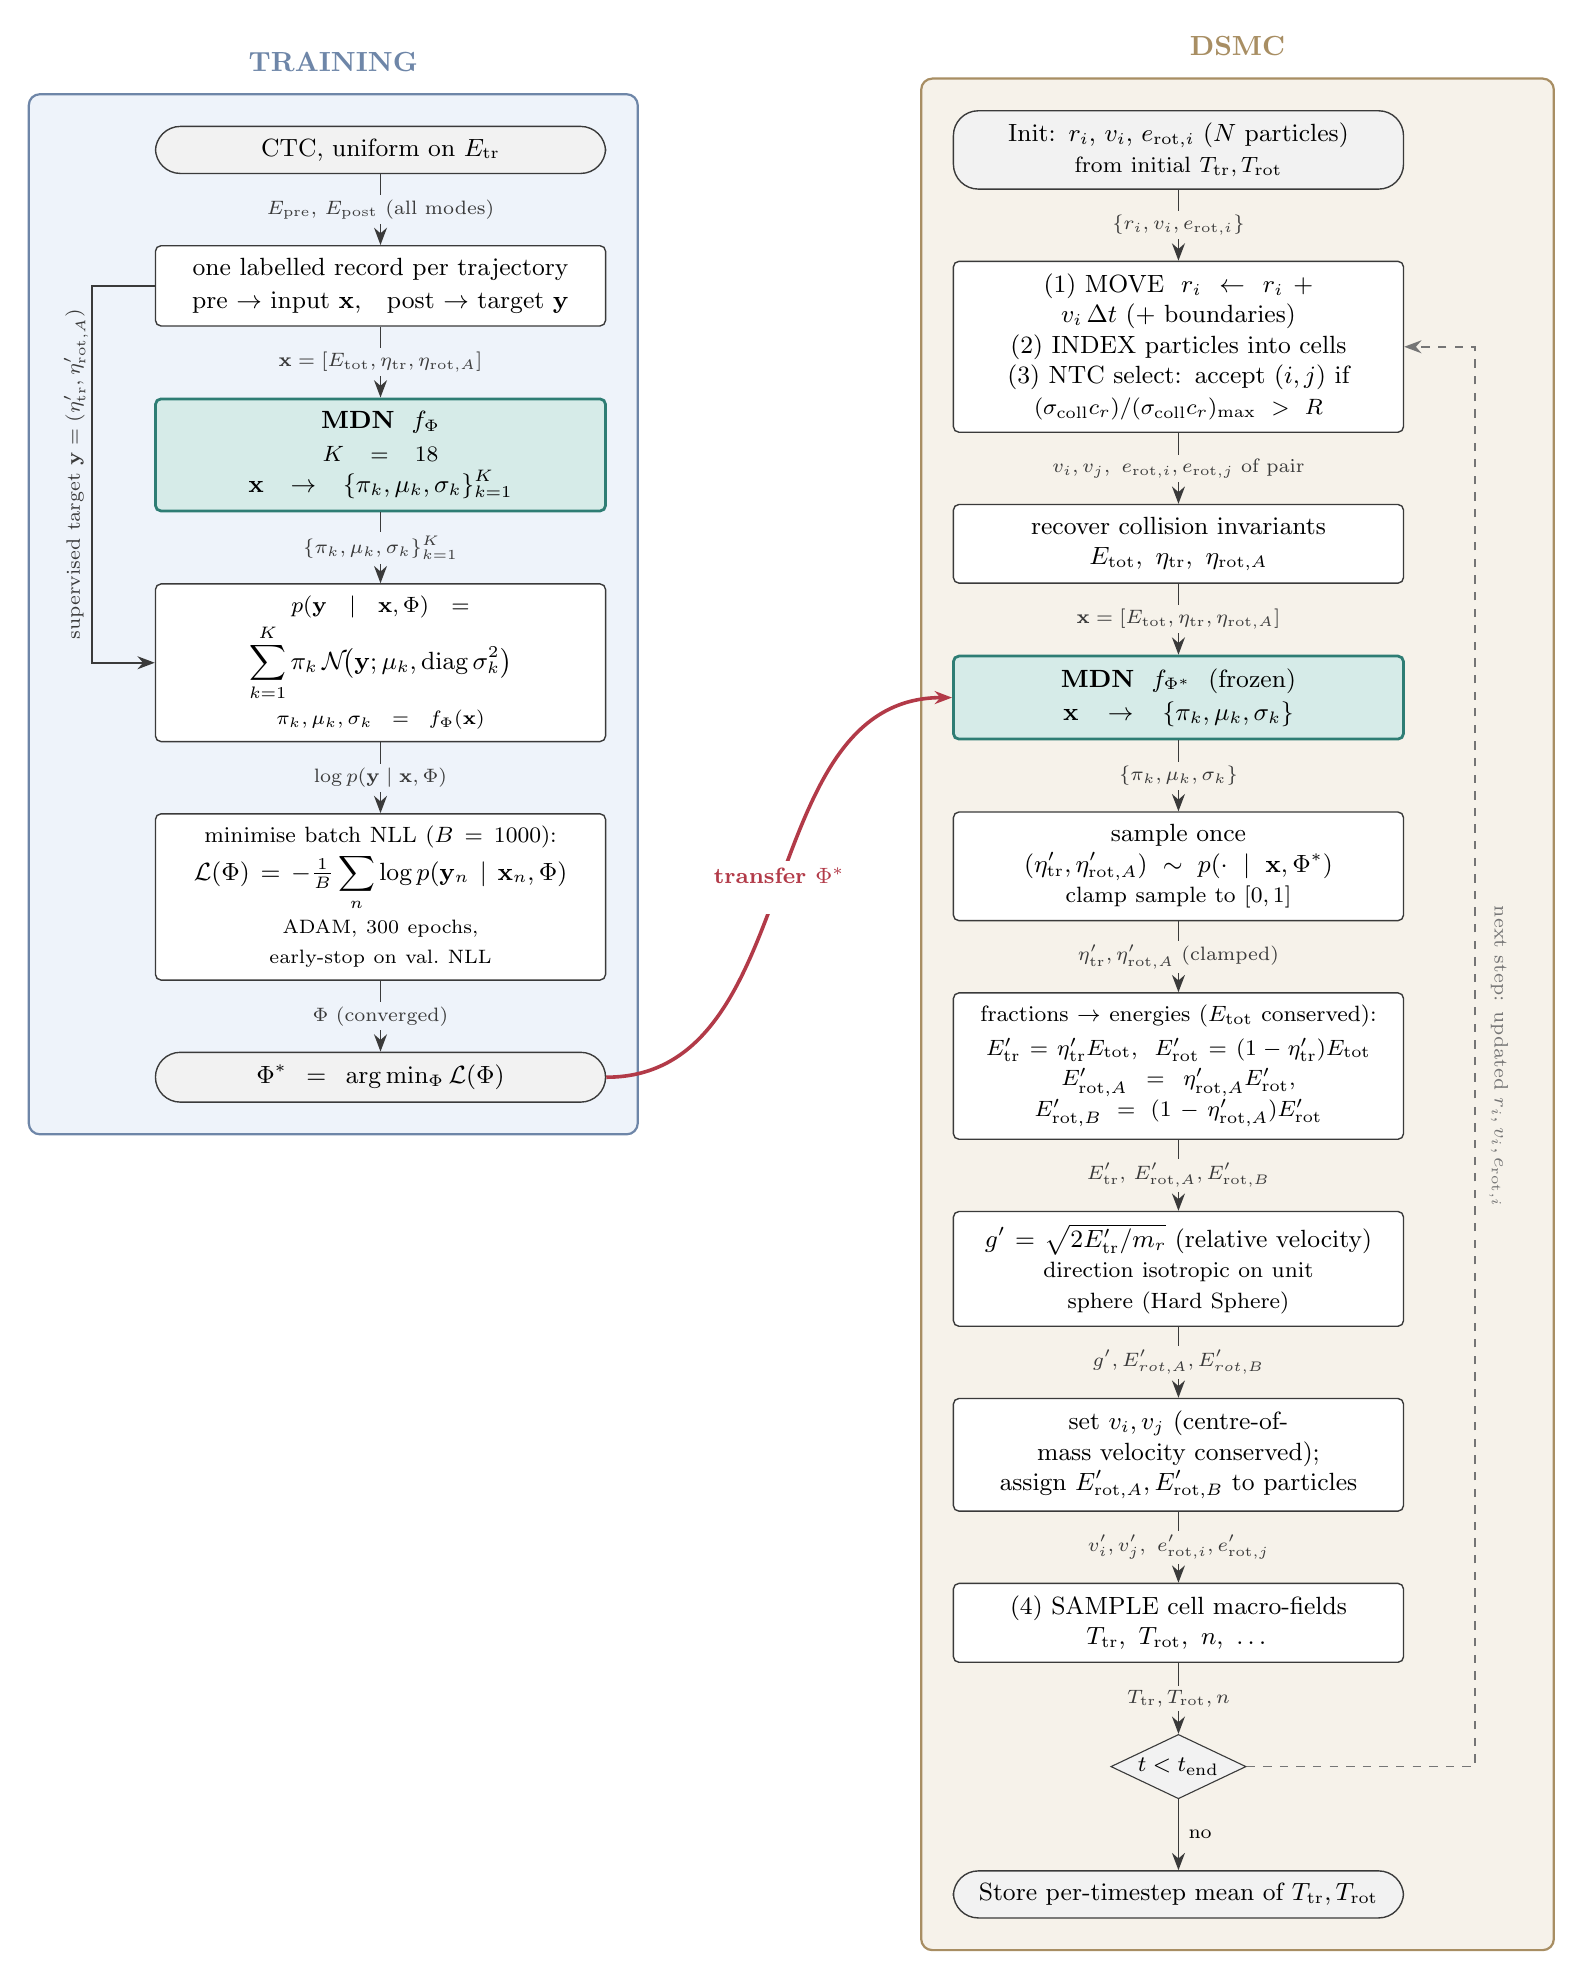
\begin{tikzpicture}[
  font=\small,
  >={Stealth[length=2.2mm]},
  node distance=9mm,
  proc/.style={rectangle, rounded corners=2pt, draw=nodeln, fill=white,
               align=center, inner sep=4.5pt, text width=54mm, line width=0.5pt},
  mdn/.style={rectangle, rounded corners=2pt, draw=mdnline, fill=mdnfill,
              align=center, inner sep=4.5pt, text width=54mm, line width=1pt},
  io/.style={rectangle, rounded corners=9pt, draw=nodeln, fill=black!5,
             align=center, inner sep=4.5pt, text width=54mm, line width=0.5pt},
  dec/.style={diamond, aspect=2.1, draw=nodeln, fill=black!5,
              align=center, inner sep=1pt, font=\footnotesize},
  arr/.style={->, draw=nodeln, line width=0.6pt},
  transfer/.style={->, draw=accent, line width=1.3pt},
  loop/.style={->, draw=nodeln!70, line width=0.6pt, dashed},
  title/.style={font=\bfseries},
  elabT/.style={midway, fill=trainbg, inner sep=1.5pt, font=\scriptsize, text=nodeln},
  elabD/.style={midway, fill=dsmcbg, inner sep=1.5pt, font=\scriptsize, text=nodeln}
]

% =================== TRAINING COLUMN ===================
\node[io] (t1) {CTC, uniform on $\Etr$};
\node[proc, below=of t1] (t2) {one labelled record per trajectory\\[1pt]
  pre $\rightarrow$ input $\xv$,\quad post $\rightarrow$ target $\yv$};
\node[mdn, below=of t2] (t5) {\textbf{MDN}\ \ $f_{\Phi}$\\[1pt]
  {\footnotesize $K=18$}\\
  $\xv\ \rightarrow\ \{\pi_k,\mu_k,\sigma_k\}_{k=1}^{K}$};
\node[proc, below=of t5] (t6) {%
  {\footnotesize $p(\yv\mid\xv,\Phi)=$}\\[1pt]
  $\displaystyle\sum_{k=1}^{K}\pi_k\,\mathcal{N}\!\big(\yv;\mu_k,\operatorname{diag}\sigma_k^2\big)$\\[2pt]
  {\scriptsize $\pi_k,\mu_k,\sigma_k=f_\Phi(\xv)$}};
\node[proc, below=of t6] (t7) {%
  {\footnotesize minimise batch NLL ($B=1000$):}\\[1pt]
  $\displaystyle \mathcal{L}(\Phi)=-\tfrac{1}{B}\sum_{n}\log p(\yv_n\mid\xv_n,\Phi)$\\[2pt]
  {\scriptsize ADAM, 300 epochs, early-stop on val.\ NLL}};
\node[io, below=of t7] (t8) {$\Phi^{*}=\arg\min_\Phi \mathcal{L}(\Phi)$};

% =================== DSMC COLUMN ===================
\node[io, right=44mm of t1] (d1) {Init: $r_i,\,v_i,\,e_{\mathrm{rot},i}$\ ($N$ particles)\\
  {\footnotesize from initial $T_{\mathrm{tr}},T_{\mathrm{rot}}$}};
\node[proc, below=of d1] (d2) {%
  (1)\ MOVE\ \ $r_i\leftarrow r_i+v_i\,\Delta t$\ (+ boundaries)\\
  (2)\ INDEX particles into cells\\
  (3)\ NTC select: accept $(i,j)$ if\\
  {\footnotesize $(\sigma_{\mathrm{coll}}c_r)/(\sigma_{\mathrm{coll}}c_r)_{\max}>R$}};
\node[proc, below=of d2] (d3) {recover collision invariants\\
  $\Etot,\ \etatr,\ \etarot$};
\node[mdn, below=of d3] (d5) {\textbf{MDN}\ \ $f_{\Phi^{*}}$\ \ (frozen)\\[1pt]
  $\xv\ \rightarrow\ \{\pi_k,\mu_k,\sigma_k\}$};
\node[proc, below=of d5] (d6) {sample once\\
  $(\etatr',\etarot')\sim p(\cdot\mid\xv,\Phi^{*})$\\
  {\footnotesize clamp sample to $[0,1]$}};
\node[proc, below=of d6] (d7) {%
  {\footnotesize fractions $\rightarrow$ energies ($\Etot$ conserved):}\\[1pt]
  {\footnotesize $\Etr'=\etatr'\Etot$,\ \ $\Erot'=(1-\etatr')\Etot$}\\
  {\footnotesize $E'_{\mathrm{rot},A}=\etarot'\Erot'$,\ \ $E'_{\mathrm{rot},B}=(1-\etarot')\Erot'$}};
\node[proc, below=of d7] (d8) {$g'=\sqrt{2\Etr'/m_r} \mathrm{\ (relative\ velocity)}$\\
  {\footnotesize direction isotropic on unit sphere (Hard Sphere)}};
\node[proc, below=of d8] (d9) {set $v_i,v_j$ (centre-of-mass velocity conserved);\\
  assign $E'_{\mathrm{rot},A},E'_{\mathrm{rot},B}$ to particles};
\node[proc, below=of d9] (d10) {(4)\ SAMPLE cell macro-fields\\
  $T_{\mathrm{tr}},\ T_{\mathrm{rot}},\ n,\ \dots$};
\node[dec, below=of d10] (d11) {$t<t_{\mathrm{end}}$};
\node[io, below=of d11] (d12) {Store per-timestep mean of $T_{\mathrm{tr}},T_{\mathrm{rot}}$};

% =================== TRAINING FLOW (labelled) ===================
\draw[arr] (t1)--(t2) node[elabT]{$E_{\mathrm{pre}},\,E_{\mathrm{post}}$ (all modes)};
\draw[arr] (t2)--(t5) node[elabT]{$\xv=[\Etot,\etatr,\etarot]$};
\draw[arr] (t5)--(t6) node[elabT]{$\{\pi_k,\mu_k,\sigma_k\}_{k=1}^{K}$};
\draw[arr] (t6)--(t7) node[elabT]{$\log p(\yv\mid\xv,\Phi)$};
\draw[arr] (t7)--(t8) node[elabT]{$\Phi$ (converged)};

% target-y rail (left side) -- solid black: it is a real variable
\coordinate (yr) at ([xshift=-8mm]t2.west);
\coordinate (yrb) at (yr |- t6.west);
\coordinate (trainL) at ([xshift=-12mm]t2.west);
\draw[arr] (t2.west) -- (yr) -- (yrb) -- (t6.west);
\node[rotate=90, font=\scriptsize, text=nodeln] at ([xshift=-2mm]$(yr)!0.5!(yrb)$)
  {supervised target $\yv=(\etatr',\etarot')$};

% =================== DSMC FLOW (labelled) ===================
\draw[arr] (d1)--(d2) node[elabD]{$\{r_i,v_i,e_{\mathrm{rot},i}\}$};
\draw[arr] (d2)--(d3) node[elabD]{$v_i,v_j,\ e_{\mathrm{rot},i},e_{\mathrm{rot},j}$ of pair};
\draw[arr] (d3)--(d5) node[elabD]{$\xv=[\Etot,\etatr,\etarot]$};
\draw[arr] (d5)--(d6) node[elabD]{$\{\pi_k,\mu_k,\sigma_k\}$};
\draw[arr] (d6)--(d7) node[elabD]{$\etatr',\etarot'$ (clamped)};
\draw[arr] (d7)--(d8) node[elabD]{$\Etr',\,E'_{\mathrm{rot},A},E'_{\mathrm{rot},B}$};
\draw[arr] (d8)--(d9) node[elabD]{$g', E_{rot,A}', E_{rot,B}'$ };
\draw[arr] (d9)--(d10) node[elabD]{$v_i',v_j',\ e_{\mathrm{rot},i}',e_{\mathrm{rot},j}'$};
\draw[arr] (d10)--(d11) node[elabD]{$T_{\mathrm{tr}},T_{\mathrm{rot}},n$};
\draw[arr] (d11)--(d12) node[midway,right,font=\scriptsize]{no};

% DSMC loop-back rail (right side, clear of the node boxes)
\coordinate (dsmcR) at ([xshift=15mm]d2.east);
\coordinate (railTop) at ([xshift=9mm]d2.east);
\draw[loop] (d11.east) -- (d11.east -| railTop) -- (railTop) -- (d2.east);
\coordinate (railMid) at ($(d11.east -| railTop)!0.5!(railTop)$);
\node[rotate=-90, font=\scriptsize, text=nodeln!70] at ([xshift=3mm]railMid)
  {next step: updated $r_i,v_i,e_{\mathrm{rot},i}$};

% =================== TRANSFER ARROW (label on white fill, no clip) ===================
\draw[transfer] (t8.east) to[out=0,in=180] (d5.west);
\node[fill=white, inner sep=2.5pt, font=\footnotesize\bfseries, text=accent, align=center]
  at ($(t8.east)!0.5!(d5.west)$)
  {transfer $\Phi^{*}$\\[-1pt]};

% =================== PANEL BACKGROUNDS + TITLES ===================
\begin{scope}[on background layer]
  \node[fill=trainbg, rounded corners=4pt, draw=trainln, line width=0.8pt,
        fit=(t1)(t8)(trainL), inner sep=4mm] (trainpanel) {};
  \node[fill=dsmcbg, rounded corners=4pt, draw=dsmcln, line width=0.8pt,
        fit=(d1)(d12)(dsmcR), inner sep=4mm] (dsmcpanel) {};
\end{scope}

\node[title, above=1.5mm of trainpanel.north, text=trainln] {TRAINING};
\node[title, above=1.5mm of dsmcpanel.north, text=dsmcln] {DSMC};

\end{tikzpicture}
\end{document}
